\section{Objective}
While explaining figues using Latex I will always suggest you to use Labels for the images. The reason is you would not know where the images willl be located after compilation (unless you use `H' as an attribute, which is not advisable). So always use labels and use them as as `\\ref'  in the expalination in that way you will need not worry about the whereabouts of the images.
This chapter deals with providing the proof of concept for the architecture and formulation proposed in chapter 2 and chapter 3 respectively.  The Software used to perform simulation is explained. The solvers like Gurobi and CPLEX which adapted to solve the combinatorial problem are briefly shown. Finally, an in-depth inference on the obtained results is given. \par

\section{Implementation Methodology}

This is a simple Algorithm using the package algorithmic. It shows binpacking used in my thesis.
Hope this helps you.



\begin{algorithm}
\SetKwFunction{KwFn}{\textbf{BestPaths}}

\KwFn{$a_s,a_d,\pi_{u,v}$}\\
\Begin{
 \ForEach{path in $\pi_{u,v}$}{
     	\ForEach {Paths in $ \pi_{u,v}$ }{
		cost[]$\leftarrow$  Calcuate Cost of Each Cost\;
	}
            \ForEach {cost in cost[]}{
	    	$\Pi_{u,v}  \leftarrow $ Path with least cost in $\pi_{u,v}$\; 
	}
}Return{ \{$\Pi_{u,v}$, cost $\Pi_{u,v}$ \}}}

\SetKwFunction{KwB}{\textbf{BinPacking}}
\KwB{$\Pi_{u,v}$}\\
\Begin{
\ForEach {link in $\Pi_{u,v}$}{
  \ForEach{ Wavelength in link}{
      AvailableWavelength[] $\leftarrow $getWavelength(link)\;
	  }
}
\ForEach{ wavelength in AvailWavelength[]}{
	compare if all the Links in path $\Pi_{u,v}$ in \\ AvailWavelength[] has the wavelength available.\\
	\eIf { available wavelengths in path $\Pi_{u,v}$ is true for all links in it}{
			Return( Selected Wavelength)\\ 
			break\;
			}{Update
\\
			$\Pi_{u,v} \leftarrow$ BestPaths$(a_s,a_d,\pi_{u,v})$}
	\If { no path found in $(a_s, a_d,\pi_{u,v})$}{
			Return Embedding Not Possible\\
			Select New VN Request
			}
		      }
	Return ( Selected Wavelength)
 }
\caption{Selecting Links and Wavelegths for between the Substrate Nodes}
\label{algo:one}
\end{algorithm} 



\section{Discussion of Results}
\subsection{Definition of Metrics Used For the Evaluation}
Always Try to create images for gray scale. Because I had hard time converting all my results from color images to gray scale images at the end. And of-course no body wants to take print out in color.   The paths where I have included images is kind of long, but you can change the paths for your convinience. 
 \begin{figure}[H]
\centering
\frame{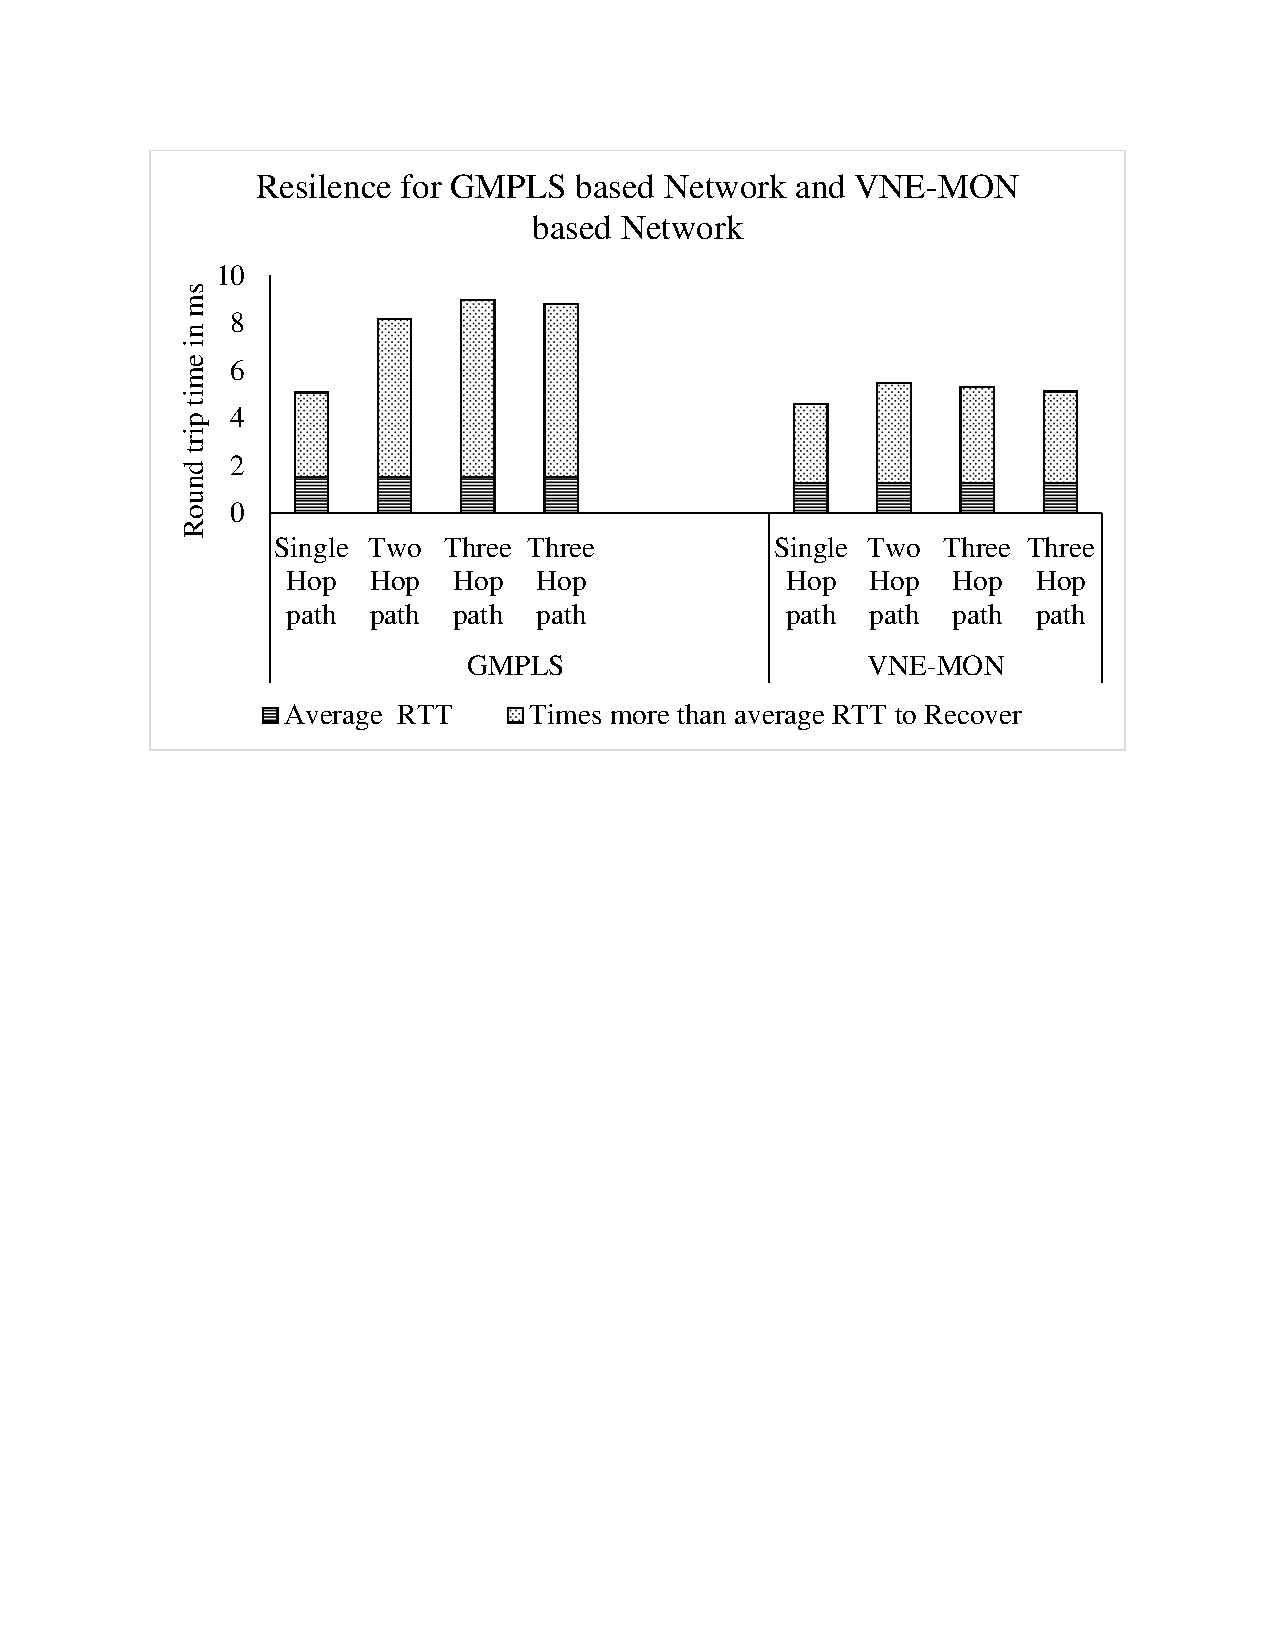
\includegraphics[clip, trim= 2.5cm 15.2cm 2.5cm 2.5cm,width=0.70\columnwidth]{Results/pdf/ResultsPDF/fourteen.pdf}}
\caption{ Cost vs. SRLG factor.}
\label{fig:before4}
\end{figure}

\section{Summary}
  